\documentclass[a4paper,11pt,twoside,DIV10,english,numbers=noendperiod]{scrbook}
\usepackage[a4paper,left=3.5cm,right=2.5cm,bottom=3.5cm,top=3cm]{geometry}
%{report}

% ~~~~~~~~~~~~~~~my packages~~~~~~~~~~~`
% Multiline comments
\usepackage{verbatim}
%\usepackage[llncsdoc]{llncsdoc}
\usepackage{makeidx}  % allows for indexgeneration

%\usepackage{fullpage}
\usepackage[english]{babel}
\usepackage{graphicx}
\usepackage{multirow}
\usepackage{rotating}
\usepackage[latin1]{inputenc}
\usepackage[numbers,square]{natbib}
\usepackage{scrhack}
%Kapitel�berschriften in Gro�buchstaben
\setkomafont{chapter}{\normalfont \scshape \Huge}
\setkomafont{section}{\normalfont \bfseries \LARGE}
\setkomafont{subsection}{\normalfont \bfseries \Large}
\setkomafont{subsubsection}{\normalfont \bfseries \large}
\setkomafont{paragraph}{\normalfont \bfseries \large}
%Pallanoid Schriftart verwenden
\usepackage{mathpazo}

%Auswahl der Schriftart erm�gliche, damit Titelpage in Times und Rest in Pazo
\usepackage[T1]{fontenc}
\newcommand{\changefont}[3]{
\fontfamily{#1} \fontseries{#2} \fontshape{#3} \selectfont}

\usepackage{scalefnt}
\usepackage{titlesec}
\usepackage{titletoc}
\titleformat{\chapter}[display]
{\mdseries\huge\scshape}
{	\filleft
	\begingroup
		\scalefont{3}
			{\bfseries{\thechapter}}
	\endgroup}
{0ex}
{%\titlerule
\vspace{1ex}%
\filright}
[\vspace{1ex}%
\titlerule]

% Leere Seite ohne Seitennummer, naechste Seite rechts
\newcommand{\blankpage}{
 \clearpage{\pagestyle{empty}\cleardoublepage}
}

% Keine einzelnen Zeilen beim Anfang eines Abschnitts (Schusterjungen)
\clubpenalty = 10000
% Keine einzelnen Zeilen am Ende eines Abschnitts (Hurenkinder)
\widowpenalty = 10000 \displaywidowpenalty = 10000

%\usepackage[pdftex]{graphicx,color}
\usepackage{amsmath,amssymb,subfigure}

% Zeilenabstand einstellen %
\renewcommand{\baselinestretch}{1.25}
%\usepackage{setspace}
%\onehalfspacing

% Floating-Umgebungen anpassen %
\renewcommand{\topfraction}{0.9}
\renewcommand{\bottomfraction}{0.8}

% Theorem-Umgebungen
\usepackage[amsmath,thmmarks]{ntheorem}

% Caption Packet
\usepackage[margin=0pt,font=small,labelfont=bf]{caption}

% URLs
\usepackage{url}

% Bibtex deutsch
%\usepackage{bibgerm}

%\usepackage{abstract}

% Algorithmen

\usepackage{float}
\usepackage[ pdftex, plainpages=false, pdfpagelabels, hypertexnames=true, linktocpage=true, bookmarksopen=true, bookmarksopenlevel=1] {hyperref}
\usepackage[chapter]{algorithm}
\usepackage{algorithmic}

\setcounter{equation}{0}
% Theorem-Optionen %
\theoremseparator{.}
\theoremstyle{change}
\newtheorem{theorem}{Theorem}[section]
\newtheorem{satz}[theorem]{Satz}
\newtheorem{lemma}[theorem]{Lemma}
\newtheorem{korollar}[theorem]{Korollar}
\newtheorem{proposition}[theorem]{Proposition}
% Ohne Numerierung
\theoremstyle{nonumberplain}
\renewtheorem{theorem*}{Theorem}
\renewtheorem{satz*}{Satz}
\renewtheorem{lemma*}{Lemma}
\renewtheorem{korollar*}{Korollar}
\renewtheorem{proposition*}{Proposition}
% Definitionen mit \upshape
\theorembodyfont{\upshape}
\theoremstyle{change}
\newtheorem{definition}[theorem]{Definition}
\theoremstyle{nonumberplain}
\renewtheorem{definition*}{Definition}
% Kursive Schrift
\theoremheaderfont{\itshape}
\newtheorem{notation}{Notation}
\newtheorem{konvention}{Konvention}
\newtheorem{bezeichnung}{Bezeichnung}
\theoremsymbol{\ensuremath{\Box}}
\newtheorem{beweis}{Beweis}
\theoremsymbol{}
\theoremstyle{change}
\theoremheaderfont{\bfseries}
\newtheorem{bemerkung}[theorem]{Bemerkung}
\newtheorem{beobachtung}[theorem]{Beobachtung}
\newtheorem{beispiel}[theorem]{Beispiel}
\newtheorem{problem}{Problem}
\theoremstyle{nonumberplain}
\renewtheorem{bemerkung*}{Bemerkung}
\renewtheorem{beispiel*}{Beispiel}
\renewtheorem{problem*}{Problem}

% Algorithmen anpassen %
\renewcommand{\algorithmicrequire}[1]{\textbf{Eingabe:}#1\\}
\renewcommand{\algorithmicensure}[1]{\textbf{Ausgabe:}#1\\}
\floatname{algorithm}{Algorithmus}
\renewcommand{\listalgorithmname}{Algorithmenverzeichnis}

%Silbentrennung
\hyphenation{De-zi-mal-trenn-zeichen In-stal-la-ti-ons-as-sis-tent Ist-Schwer-punkt-po-si-tion}

\newcommand{\modelica}[3]{\vspace*{.75cm}
													\begin{addmargin}[0.5cm]{0.5cm} 
														\begin{minipage}{\linewidth}
															\noindent\rule[1ex]{\textwidth}{1pt}\\
															\noindent{\textbf{#1}\hfill\footnotesize(\textit{Modelica}-Quelltext - Auszug aus \ref{#2} auf Seite \pageref{#2})\normalsize}\\
															\noindent\rule[1ex]{\textwidth}{1pt}														
															\begin{flushleft}
																\hangindent=0.5cm #3	\\
															\end{flushleft}															
															\noindent\rule[1ex]{\textwidth}{1pt}\\
														
														\end{minipage}
													\end{addmargin}
													%\vspace*{.75cm}
												 }

\begin{document}
%\raggedbottom
	%\frontmatter

	\setcounter{secnumdepth}{3}
	\setcounter{tocdepth}{3}

	%\pagestyle{headings}  % switches on printing of running heads
	\pagenumbering{roman}
	
	%Schriftart f�r Titelseite auf TIMES
	\changefont{ptm}{m}{n}
	
	
\begin{titlepage}

 \sffamily

 \vspace*{-2cm}

 \begin{minipage}{0.48\linewidth}
  
\includegraphics[width=1.0\textwidth]{Bilder/tud_logo_rgb}
 \end{minipage}
 
 \vspace*{1.7cm}
 \begin{center}
  \noindent{
 \begin{minipage}{0.55\linewidth}
	\hrulefill
  \vspace{2.0cm}
 \end{minipage}}
 \hfil
 \begin{minipage}{0.4\linewidth}
  % empty
 \end{minipage}
 \begin{minipage}{0.15\linewidth}
  % empty
 \end{minipage}
 \hfil
 \begin{minipage}{0.55\linewidth}
  \begin{center}
    \Large\textbf{Master Thesis}
  \end{center}
  \begin{center}
    \large{Estimation of Underactuated Degrees of Freedom(DOF's) in Humanoid Robots}\\[3ex]
  \end{center}
  \vspace{0.75cm}
  \begin{center}
    \normalsize{Rajesh Rajendran}\\
 
 \small{rajesh.rajendran@tu-dortmund.de}\\[2ex]
    \large{\today}
  \end{center}
 \end{minipage}
 \hfil
 \begin{minipage}{0.05\linewidth}
  % empty
 \end{minipage}
 \begin{minipage}{0.55\linewidth}
 \vspace{2.0cm}
  \hrulefill
 \end{minipage}
 \end{center}
 \vspace*{2cm}

 \vfill
 			\rmfamily
 			\changefont{ppl}{m}{n}
 			\begin{table} [H]
				\centering
				\normalsize
				\begin{tabular}{p{0.53\textwidth}p{0.41\textwidth}}
					Examiner: & \\
					Name of first examiner & Name of second examiner\\
			  	&\\	
			  	Abteilung Informationstechnik\newline Institut f\"{u}r Roboterforschung  & Lehrstuhl des Zweitgutachters\newline Fakult\"{a}t f\"{u}r Informatik\\

			  \end{tabular}
			 \end{table}
			 
				\rmfamily
 				\changefont{ppl}{m}{n}

 \end{titlepage}
 
    %Schriftart wieder zur\"{u}ck auf pazo
    \changefont{ppl}{m}{n}



    \blankpage
    \newpage
    \tableofcontents
    \cleardoublepage

    \pagenumbering{arabic}
    \parindent 0pt
    % Buchstaben in Formeln bzw. Gleichungen sollten
% in einer Arbeit durchweg die gleiche Bedeutung haben.
% Um das zu unterst�tzen, die Schreibarbeit zu verringern,
% und Umbennungen zu vereinfachen sollten alle Bezeichner
% zentral in einer Datei als Makro definiert werden.

% Abk�rzungen
\newcommand{\IRF}{Institut f�r Roboterforschung}

% Formelvariablen
\newcommand{\Ri}[2]{R^{#1}_{#2}} % Rotationsmatrix von Frame #2 zu Frame #1
\newcommand{\Rv}[2]{R_v\left(#1, #2\right)} % Rotationsmatrix um beliebige Achse #1 bei Winkel #1

    % Diese Datei dient als Testseite für Befehle oder Formeln. 
% Alle hier eingegebenen können direkt am Anfang der Arbeit betrachtet werden.

%\begin{figure}
%\begin{center}
%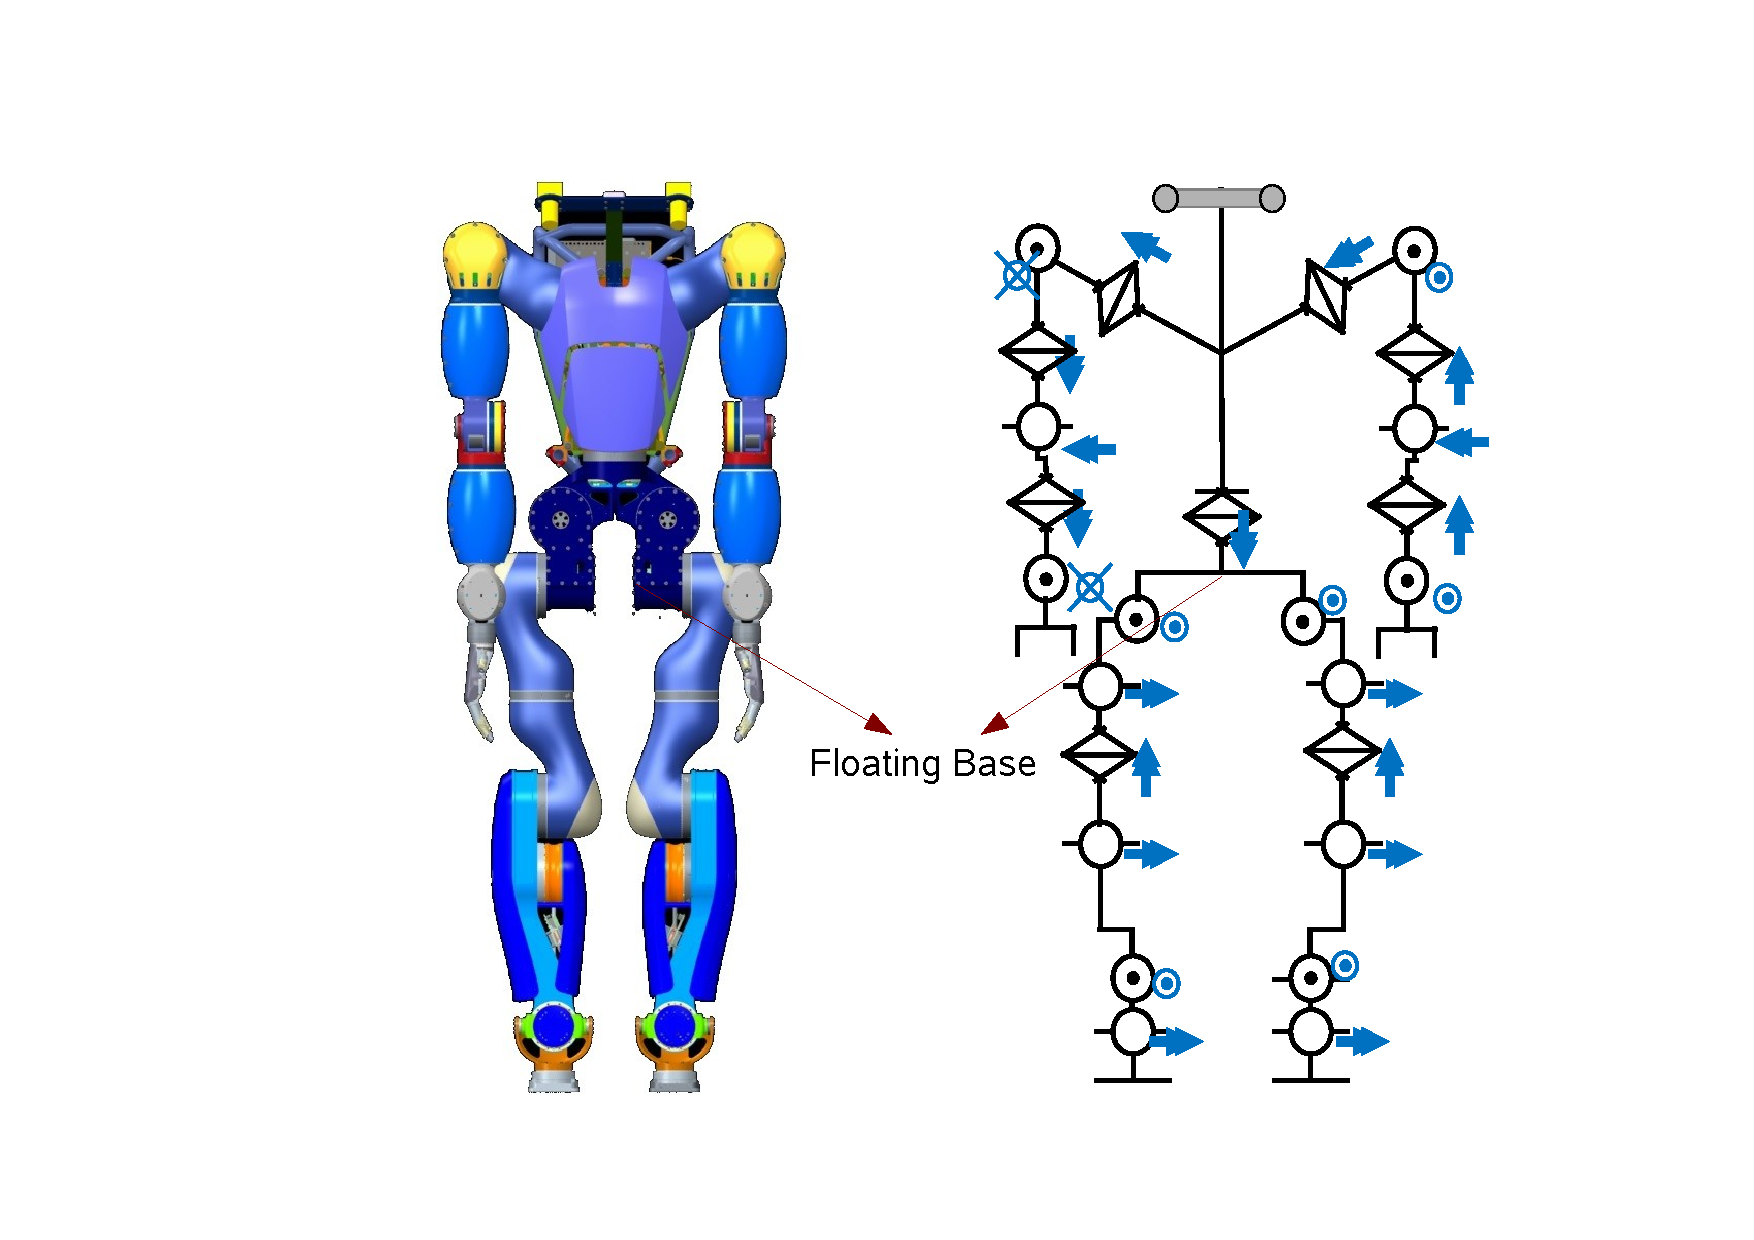
\includegraphics[scale=0.75]{Bilder/TORO_kinematic.pdf}
%\caption{test}
%\label{fig:foo}
%\end{center}
%\end{figure}
\begin{figure}
\tikzstyle{block} = [draw, fill=blue!20, rectangle, 
    minimum height=3em, minimum width=6em]
\tikzstyle{sum} = [draw, fill=blue!20, circle, node distance=1cm]
\tikzstyle{input} = [coordinate]
\tikzstyle{output} = [coordinate]
\tikzstyle{pinstyle} = [pin edge={to-,thin,black}]
\def\blockdist{2.3}
% The block diagram code is probably more verbose than necessary
\begin{tikzpicture}[auto, node distance=4cm,>=latex']
    % We start by placing the blocks
    \node [input, name=input] {};
    \node [sum, right of=input] (sum) {};
    \node [block, right of=sum] (controller) {Controller};
    \node [block, right of=controller, pin={[pinstyle]above:Disturbances},
            node distance=5cm] (system) {System};
    % We draw an edge between the controller and system block to 
    % calculate the coordinate u. We need it to place the measurement block. 
    \draw [->] (controller) -- node[name=u] {$u$} (system);
    \node [output, right of=system] (output) {};
    \node [block, below of= controller] (measurements) {Estimator};

    % Once the nodes are placed, connecting them is easy. 
    \draw [draw,->] (input) -- node {$r$} (sum);
    \draw [->] (sum) -- node {$e$} (controller);
    \draw [->] (system) -- node [name=y] {$y$}(output);
    \draw [->] (y) |- (measurements.base east);
    \draw [->] (u) |- (measurements.10);
    \draw [->] (measurements) -| node[pos=0.99] {$-$} 
        node [near end] {$\hat{x}$} (sum);
\end{tikzpicture}

\caption{Structure of state feedback controller}
\end{figure}

    %%%%%%%%%%%
    % Kapitel %
    %%%%%%%%%%%

    \chapter{Introduction}
\label{sec:einleitung}
The field of \emph{Robotics} have seen a tremendous development since the introduction of the term by \emph{Isaac Asimov} in 1940s. The fundamental components of robotic systems are mechanical structure, actuators, sensors and controller. Robotic systems range from simple \emph{Cartesian manipulator} to the complex \emph{Humanoids}. \emph{Industrial robots} are robots that are used in applications such as palletizing, material loading and unloading, part sorting, packaging etc. These robots usually operate in the structured environment whose geometrical or physical characteristics are known a priori. They are preprogrammed to execute the set of tasks. These robots have largely aided the automation of manufacturing processes in the industries. \emph{Mobile robots} that are used in the environments where human beings can hardly survive or be exposed to unsustainable risks are called \emph{Field robots}. These robots normally operate in the unstructured environments, where the geometry or physical characteristics are not known a priori. The mars rover \emph{Curiosity} is one such example. Locomotion in these robots is achieved either by wheels or by mechanical legs. The robots that navigate with mechanical legs are gaining importance, because they can navigate through the rugged terrain. The legged robots are biologically inspired structures equipped with six (hexapod-inspired from insects), four (quadrapod-inspired from animals) and two (biped-inspired from human) legs. The bipeds having the same kinematic structure as the humans are called \emph{Humanoids}. \emph{Toro (Torque controlled robot)} is the humanoid developed by Department of Robotics and Mechatronics at DLR. It is used as a platform to test advanced control concepts used for waling and balancing. \emph{Toro} was built as a biped walker shown in Figure \ref{fig:toro_biped}. Later in 2012 it have been equipped with the upperbody and hands and evolved into a humanoid. The present form of \emph{Toro} is shown in \ref{fig:toro_humanoid}.
\begin{figure}
	\centering
	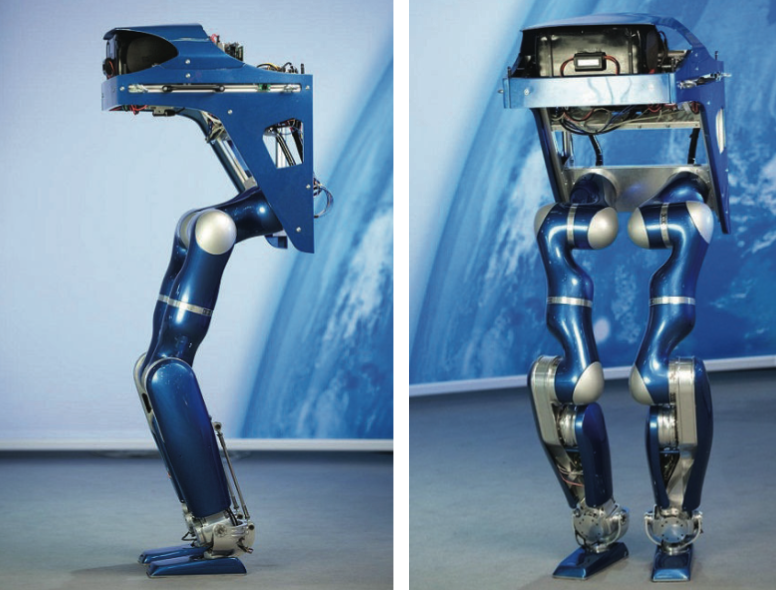
\includegraphics[scale=0.25]{Bilder/toro-biped}
	\caption{\emph{Toro} in biped form}
	\label{fig:toro_biped}
\end{figure}
\begin{figure}
\centering
	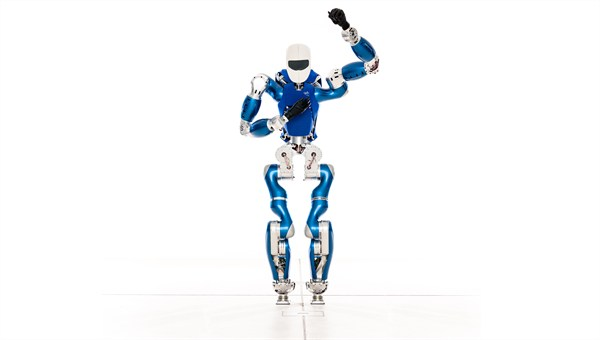
\includegraphics[trim=40mm 0mm 40mm 0mm,clip,scale=1]{Bilder/toropic}
	\caption{\emph{Toro} in humanoid form}
	\label{fig:toro_humanoid}
\end{figure}

\section{Motivation}
\begin{figure}
	\centering
	%\includegraphics[angle=-90,scale=0.65]{Bilder/walking_ctrl.pdf}
	%\pgfdeclarelayer{background}
%\pgfdeclarelayer{foreground}
%\pgfsetlayers{background,main,foreground}

% Define a few styles and constants
\tikzstyle{smallbox}=[draw, top color=white, bottom color=blue!20, text width=5em,text centered, minimum height=2.5em]
\tikzstyle{relationship} = [diamond,top color=white,bottom color=red!20,draw=red!50!black!100]
\tikzstyle{bigbox} = [smallbox,top color=white,fill=green!30,minimum height=25em,rounded corners]
\tikzstyle{input} = [coordinate]
\tikzstyle{sum} = [draw, fill=blue!20, circle, node distance=1cm]
\tikzstyle{output} = [coordinate]
\def\blockdist{3}
\def\edgedist{1.5}

\begin{tikzpicture}[node distance=2cm]
	\node (zmp)[smallbox] {ZMP};
	\node (com) [smallbox,below of=zmp,node distance=7cm] {COM};
	\node (zmp_sum) [sum,right of=zmp,node distance=3cm]{};
	\node (zmp_ctrl) [smallbox,below of=zmp_sum,node distance=2cm]{ZMP Controller};
	\node (ctrl_sum) [sum,below of=zmp_ctrl,node distance=1.5cm]{};
	\node (kin_res) [smallbox,right of=ctrl_sum,node distance=3cm]{Kinematic Resolution of COM Jacobian};
	\node (jnt_sum) [sum,right of=kin_res,node distance=2cm]{};
	\node (jnt_msr) [input,below of=jnt_sum,node distance=3.5cm]{};
	\node (zmp_calc) [smallbox,right of=zmp_sum,node distance=3cm]{ZMP Calculation};
	\node (com_div) [output,right of=com,node distance=1.5cm]{};
	\node (dxdt) [rectangle,fill=blue!20,above of=com_div,node distance=0.75cm]{$\frac{d}{dt}$};
	\node (com_sum) [sum,below of=zmp_sum,node distance=7cm]{};
	\node (com_ctrl) [smallbox,above of=com_sum,node distance=2cm]{COM Controller};
	\node (com_calc) [smallbox,below of=zmp_calc,node distance=7cm]{COM Calculation};
	\node (jnt_ctrl) [smallbox,right of=jnt_sum,node distance=1.5cm]{Joint Controller};
	\node (robot) [bigbox,right of=jnt_ctrl,node distance=2.5cm]{Real Biped Robot};
	
	\draw [->] (zmp) --node[above,pos=0.5]{\small{Des. ZMP}}(zmp_sum)node[below,pos=0.3]{$p^d$};
	\draw [->] (zmp) --node{}(com);
	\draw [-] (com) --node{}(com_div);
	\draw [->] (com_div) --node[below,pos=0.4]{\small{Des. COM}}node[above]{$c^d$}(com_sum);
	\draw [->] (com_calc) --node[below,pos=0.5]{\small{Act. COM}}node[above,pos=0.5]{$c$}node[above,pos=0.9]{$-$}(com_sum);
	\draw [->] (com_div) --node{}(dxdt);
	\draw [->] (com_sum) --node{}(com_ctrl);
	\draw [->] (dxdt) |-node[left,pos=0.3]{$\dot c^d$}(ctrl_sum);
	\draw [->] (com_ctrl) --node{}(ctrl_sum);
	\draw [->] (zmp_ctrl) --node[right,pos=0.9]{$-$}(ctrl_sum);
	\draw [->] (ctrl_sum) --node[above,pos=0.5]{\small{Control}}node[below,pos=0.5]{\small{input }$u_i$}(kin_res);
	\draw [->] (zmp_sum) --node{}(zmp_ctrl);
	\draw [->] (zmp_calc) --node[above]{\small{Act. ZMP}}node[below]{$p$}node[below,pos=0.9]{$-$}(zmp_sum);
	\draw [->] (kin_res) --node[below]{$q_d$}(jnt_sum);
	\draw [->] (jnt_sum) --node{}(jnt_ctrl);
	\draw [->] (jnt_msr) --node[left]{$q$}node[left,pos=0.9]{$-$}(jnt_sum);
	\draw [->] (jnt_ctrl)--node{}(robot);
	\draw [->] (robot.west)+(0,3.5) --node[above]{FTS}(zmp_calc.east);
	\draw [->] (robot.west)+(0,-3.5) --node[above,pos=0.3]{Joint Angles}node[below]{$q$}(com_calc);
	
	\end{tikzpicture}

	\vspace{0.5cm}
	\caption{A walking controlled scheme of humanoid robot}
	\label{fig:walk_ctrl}
\end{figure}
% Navigating the humanoids in the unknown environments and dynamic balancing of mechanical structure demands advanced control schemes. \\
The walking control of a humanoid requires the trajectory tracking while maintaining the dynamic balance of the whole structure. The Figure \ref{fig:walk_ctrl} shows a Zero moment point (ZMP) based humanoid walking control scheme \citep{choi07}. Zero moment point is a point on the surface of the foot about which the combination of inertial forces and gravity forces does not produce any net moment. It is useful for determining the dynamic stability of the robot. The ZMP of a foot is computed from the ground reaction forces measured by the FTS [Appendix \ref{sec:zmp}]. The COM in the Figure \ref{fig:walk_ctrl} represents the center of mass of the object. In this control scheme the trajectory tracking is done by controlling the COM, and the dynamic balance is maintained by controlling the ZMP of the robot. The ZMP and COM controllers are the high level controllers that drives the Kinematic resolution of COM block which computes the desired joint angles $q_d$. The joint angles are controlled by a low level joint controller.

\paragraph{Illustartion:}    
     \begin{figure}
	    \centering
    	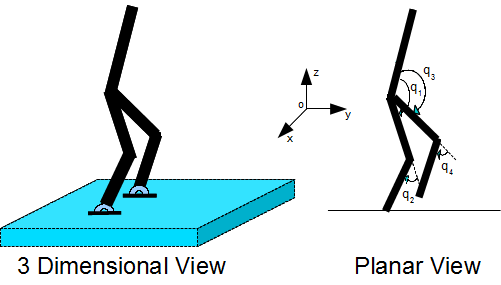
\includegraphics[scale=0.75]{Bilder/robot_flatfloor}
	    \caption{Humanoid robot standing on flat surface}	
	    \label{fig:flat_floor}
    \end{figure}
   Figure \ref{fig:flat_floor} shows a simplified two dimensional version of a humanoid robot standing on the flat surface. The COM of the robot is 
    \begin{equation}
    \label{eq:fwkin_flat}
    COM = f(q_1,q_2,q_3,q_4),
    \end{equation}
    where $f()$ is the forward kinematic function that determines the position of COM based on the joint anglse $q_i$. 
    \begin{figure}
	    \centering
    	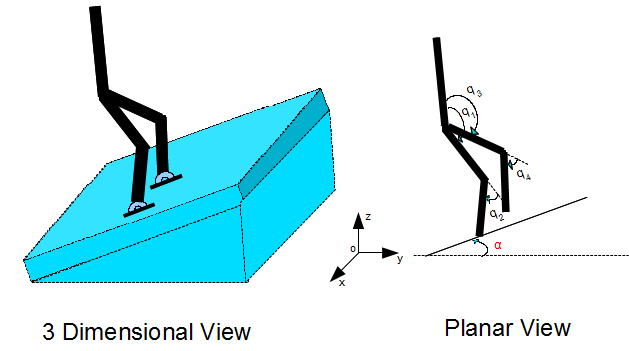
\includegraphics[scale=0.65]{Bilder/robot_slope}
	    \caption{Humanoid robot standing on a slope}	
	    \label{fig:slope}
    \end{figure}
The Figure \ref{fig:slope} shows a humanoid robot standing on the sloping surface. %In this case the COM computed by the forward kinematics function in Equation \ref{eq:fwkin_flat} will be wrong. 
%As we can see in the Figure \ref{fig:slope} there is an additional angle $\alpha$ acting between the surface of the real ground and the slope. There is no direct measurement available for this under-actuated degree of freedom. Failure to estimate this angle may lead to  tilting over an edge which might cause the robot to fall on the ground. Estimating this angle will help to achieve good balancing in the humanoid robot.
 The COM of the robot in Figure \ref{fig:slope} is given by $$COM = f(q_1,q_2,q_3,q_4,\alpha).$$  The angle $\alpha$ made by the robot with respect to the spatial frame (world coordinate frame) $O$ is not known. The computation of COM as a based on joint angles in Equation \ref{eq:fwkin_flat} will be incorrect in this case. Ignoring the angle $\alpha$ for COM computation will cause malfunctioning of the COM controller in Figure \ref{fig:walk_ctrl} and produces wrong control inputs $u_i$. The kinematic resolution of COM Jacobian block computes the desired joint angles $q_d$ assuming the robot is standing on a flat surface. When this joint trajectory executed by the controller it will cause the robot to tilt backwards. This will eventually lead to failure of the whole control scheme. This scenario motivates us to estimate the angle $\alpha$ in order to achieve robust control.  

\section{Problem Statement}
%    The focus of this thesis is estimation of under-actuated degrees of freedom of a humanoid robot.  Degrees of freedom of a robot is the number of joints present in the robot \citep{mur94}. In contrast to fixed base manipulators where the degrees of freedom is equal to number of joints in robot, the degrees of freedom of a humanoid robot is equal to sum of number of joints and degrees of freedom of a single rigid body. The under-actuated degrees of freedom of a humanoid robot are the degrees of freedom of a  rigid body.  A rigid body in three dimensional space can exhibit translational motion along \textbf{X,Y,Z} axes and rotational motion around these axes namely \emph{ roll, pitch ,yaw} as shown in Figure \ref{fig:rbody} in Chapter \ref{ch:multi_mdl}. 
	The angle $\alpha$ in Figure \ref{fig:slope} is the underactuated degree of freedom of the robot. 
% \paragraph{Underactuated degrees of freedom:}
    The term "underactuated degrees of freedom" means these degrees of freeodom are uncontrolled. They are the number of independent motions that can be exhibited by an object. For example in a two dimension (2D) space any object has 3 degrees of freedom, the object can translate along $X$ and $Y$ axes and rotate around $Z$ axis. The underactuated degrees of freedom are powered by the external forces acting on the object. For example the gravitational force makes the moon to rotate around the earth. It is not possible to directly control these degrees of freedom \citep{sab00}. In the industrial manipulators these degrees of freedom are constrained (by fixing the base to the ground), inorder to avoid complexity in control.
%%%%%%%%%%%%%%%%%%%%%%%%%%%%%%%%%%%%%%%%%%%%%%%%%%%%%%
 \begin{comment}
    \begin{figure}
    \begin{center}
    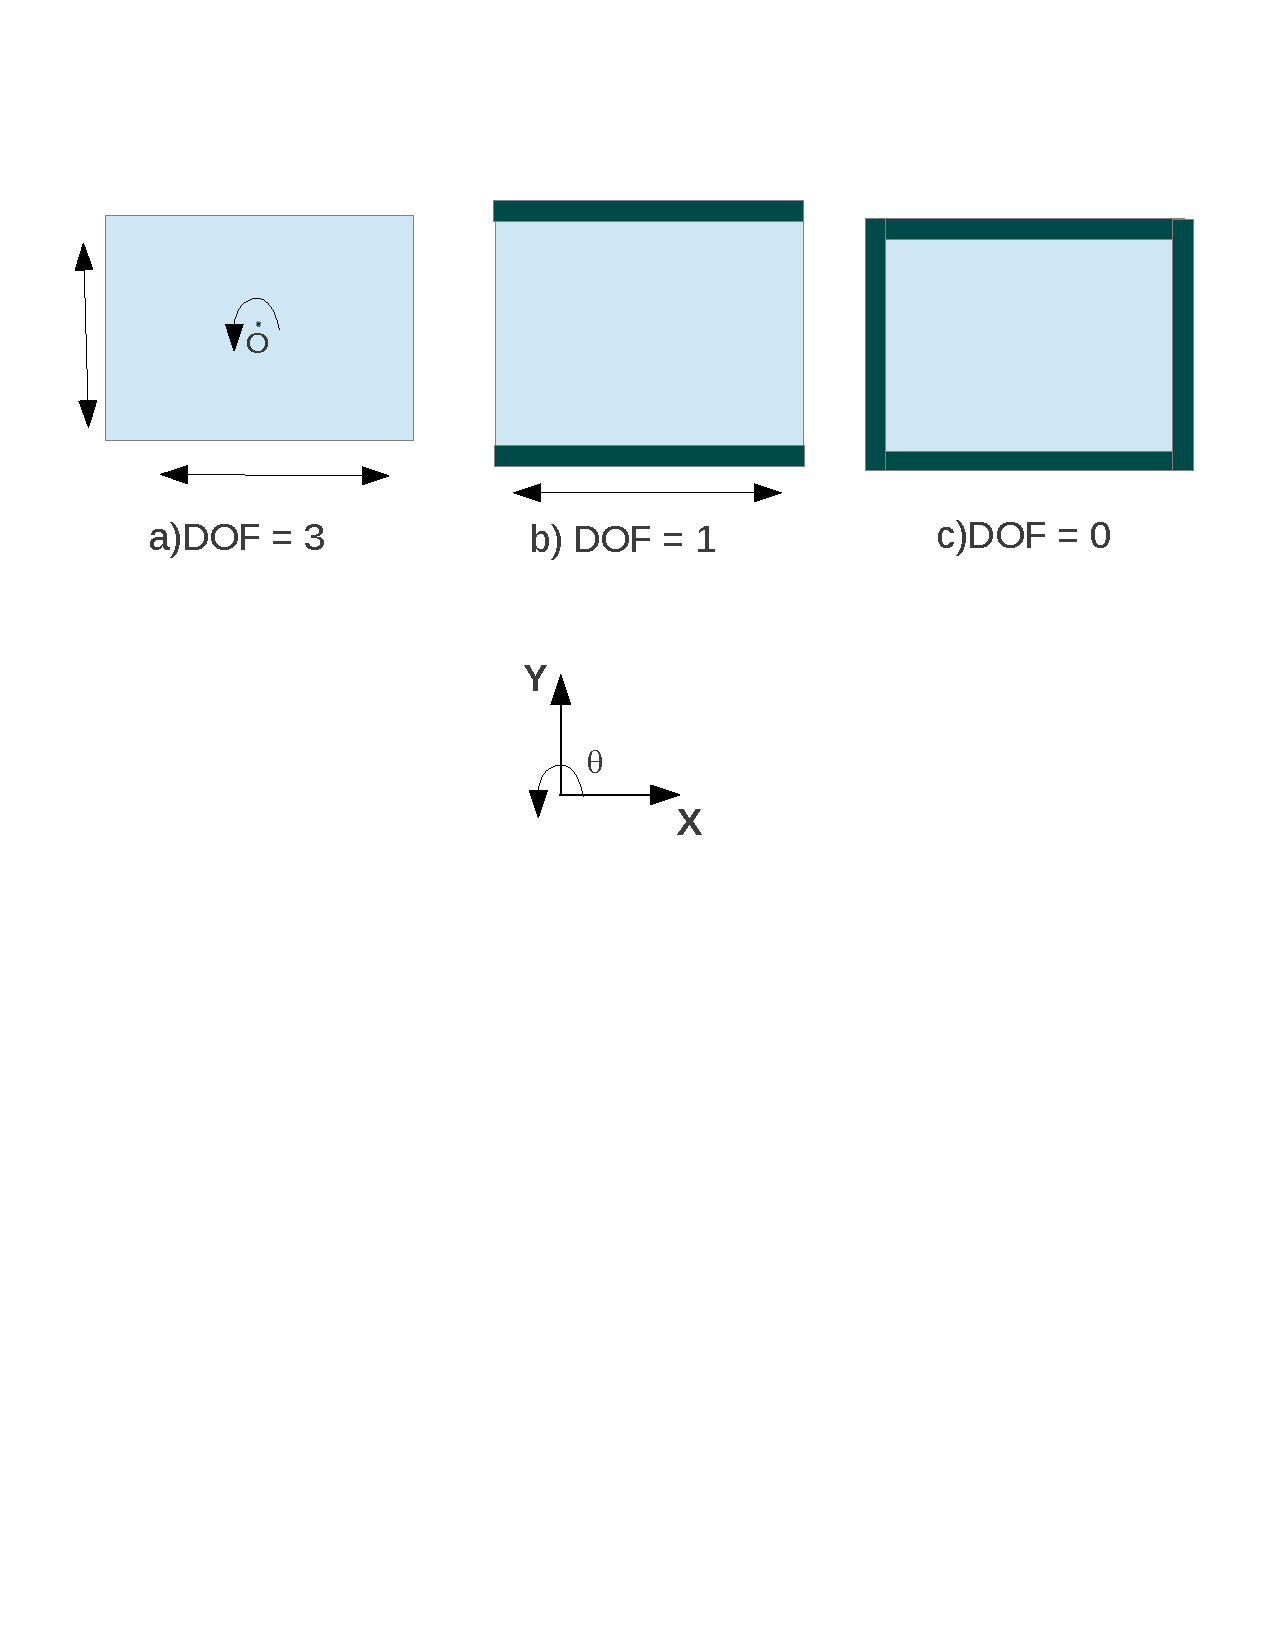
\includegraphics[trim = 10mm 130mm 10mm 20mm, scale = 0.75 ]{Bilder/dof2d.pdf}
    \caption{ Degrees of freedom of two dimensional object}
    \label{fig:dof_2d}
    \end{center}
    \end{figure}
    Figure \ref{fig:dof_2d} show how an object loses its degrees of freedom when it is constrained in 2 dimension space. In Figure \ref{fig:dof_2d} a) represents the unconstrained rectangular object free to move in space, b) represents the rectangular object constrained to move only along x axis and c) represents fully constrained rectangular object. 
    \end{comment}
%%%%%%%%%%%%%%%%%%%%%%%%%%%%%%%%%%%%%%%%%%%%%%%%%%%%%%%%%%%    
    %The ZMP of a foot is computed from the ground reaction forces measured by the FTS [Appendix \ref{sec:zmp}]. 
     
   The humanoid robots operates in a three dimensional (3D) space. The number of underactuated degrees of freedom of a 3D space is 6. 
   %When a humanoid is freely suspended (it is floating in air) it has six free degrees of freedom. But when it is constrained to its environment, the number of degrees of freedom decreases. 
   In this thesis we aim to estimate the motion of these degrees of freedom of a humanoid robot. The underactuated degrees of freedom are associated with a coordinate frame attached to the robot. In \emph{Toro} the coordinate frame is attached to the hip. As a result the state estimation problem involves estimating the motion of the hip coordinate frame. The motion parameters estimated are the position $p$, orientation $\theta$ and the body velocity $V^b$.

 \section{Methodology} 
The Kalman filter is an optimal state estimator for linear systems. The popular nonlinear extensions of Kalman filters used in practice are Extended Kalman filter(EKF) and Unscented Kalman filter(UKF). The usage of EKF for state estimation in humanoids is discussed in \citep{atk12}. \citep{bloe12} uses the EKF for state estimation in the hexapod robot. \citep{oli12} uses UKF for state estimation in humanoid robot. \citep{edg03} uses UKF for tracking the orientation of an inertial measurement unit. In this thesis the estimation problem is solved in both versions of Kalman filter. The results are compared based on accuracy of estimates and simulation time. Chapter \ref{ch:st_est} gives brief introduction to state estimation and describes the Kalman filtering algorithm. EKF and UKF algorithms are presented in Chapter \ref{ch:st_est}.

    Two different models are used for state estimation. They are the multibody system model and a simple model of  inertial measurement unit(IMU) \citep{bloe12}. The multibody system is a modelling formalism that is used to model the dynamic behaviour of a group of rigid bodies connected together to form the system. The state estimation problem using multibody system formulation is discussed in \citep{atk12}. In \citep{atk12}, the multibody system model of a simplified planar humanoid robot is used for predicting the states ahead of time. \citep{oli12} uses a multibody system model of the robot modelled using a maximal coordinate formulation scheme. The state estimation is performed separately on each link of the robot. Then the constraints due to the joints and contact are imposed on the estimates to get the true estimate of states. In this thesis, \emph{Toro} is modelled as a multibody system using minimum coordinate formulation or generalized coordinate formulation. State estimation of the multibody system involves estimation of position and velocity of the generalized coordinates. For instance, the model of \emph{Toro} have 31 generalized coordinates. The result of estimation problem will be 31 positions and 31 velocities of the generalized coordinates. Chapter \ref{ch:multi_mdl} deals with the modelling of multibody systems and its implementation in Kalman filtering algorithm. 
    
    A simplified motion model of IMU is discussed in \cite{bloe12}. In this paper, the EKF is used as sensor fusion algorithm for fusing IMU information with the kinematics of the hexapod. \citep{vis12} describes about an on-board odometry filter. The EKF is used to fuse the IMU motion model with the visual odometry and the kinematic odometry. The odometry filter is combined with vision based SLAM to obtain improved estimate of the motion model. An approach similar to \cite{bloe12} is implemented for humanoid robots. It is dealt in Chapter \ref{ch:simp_mdl}. The state estimation using this model involves predicting the position, orientation, translational velocity of the IMU sensor ahead of time. The position, orientation estimated are the under-actuated degrees of freedom and of the humanoid robot. This predicted states are updated by the kinematic information about the leg. State estimation using this model is more simpler than the multibody system. It is practically implemented on \emph{Toro}.

    \chapter{Grundlagen}
\label{sec:Grundlagen}

    \chapter{State Estimation}
\label{ch:st_est}
The state estimation is the principle of estimating the internal state(s) of the system from the measurement of input(s) and output(s) of the system. The knowledge of the internal state of the system will make the system easier to control. Figure \ref{fig:observer} shows the setup of state estimator in state feedback control loop.
\begin{figure}[h]
%  \centering
%  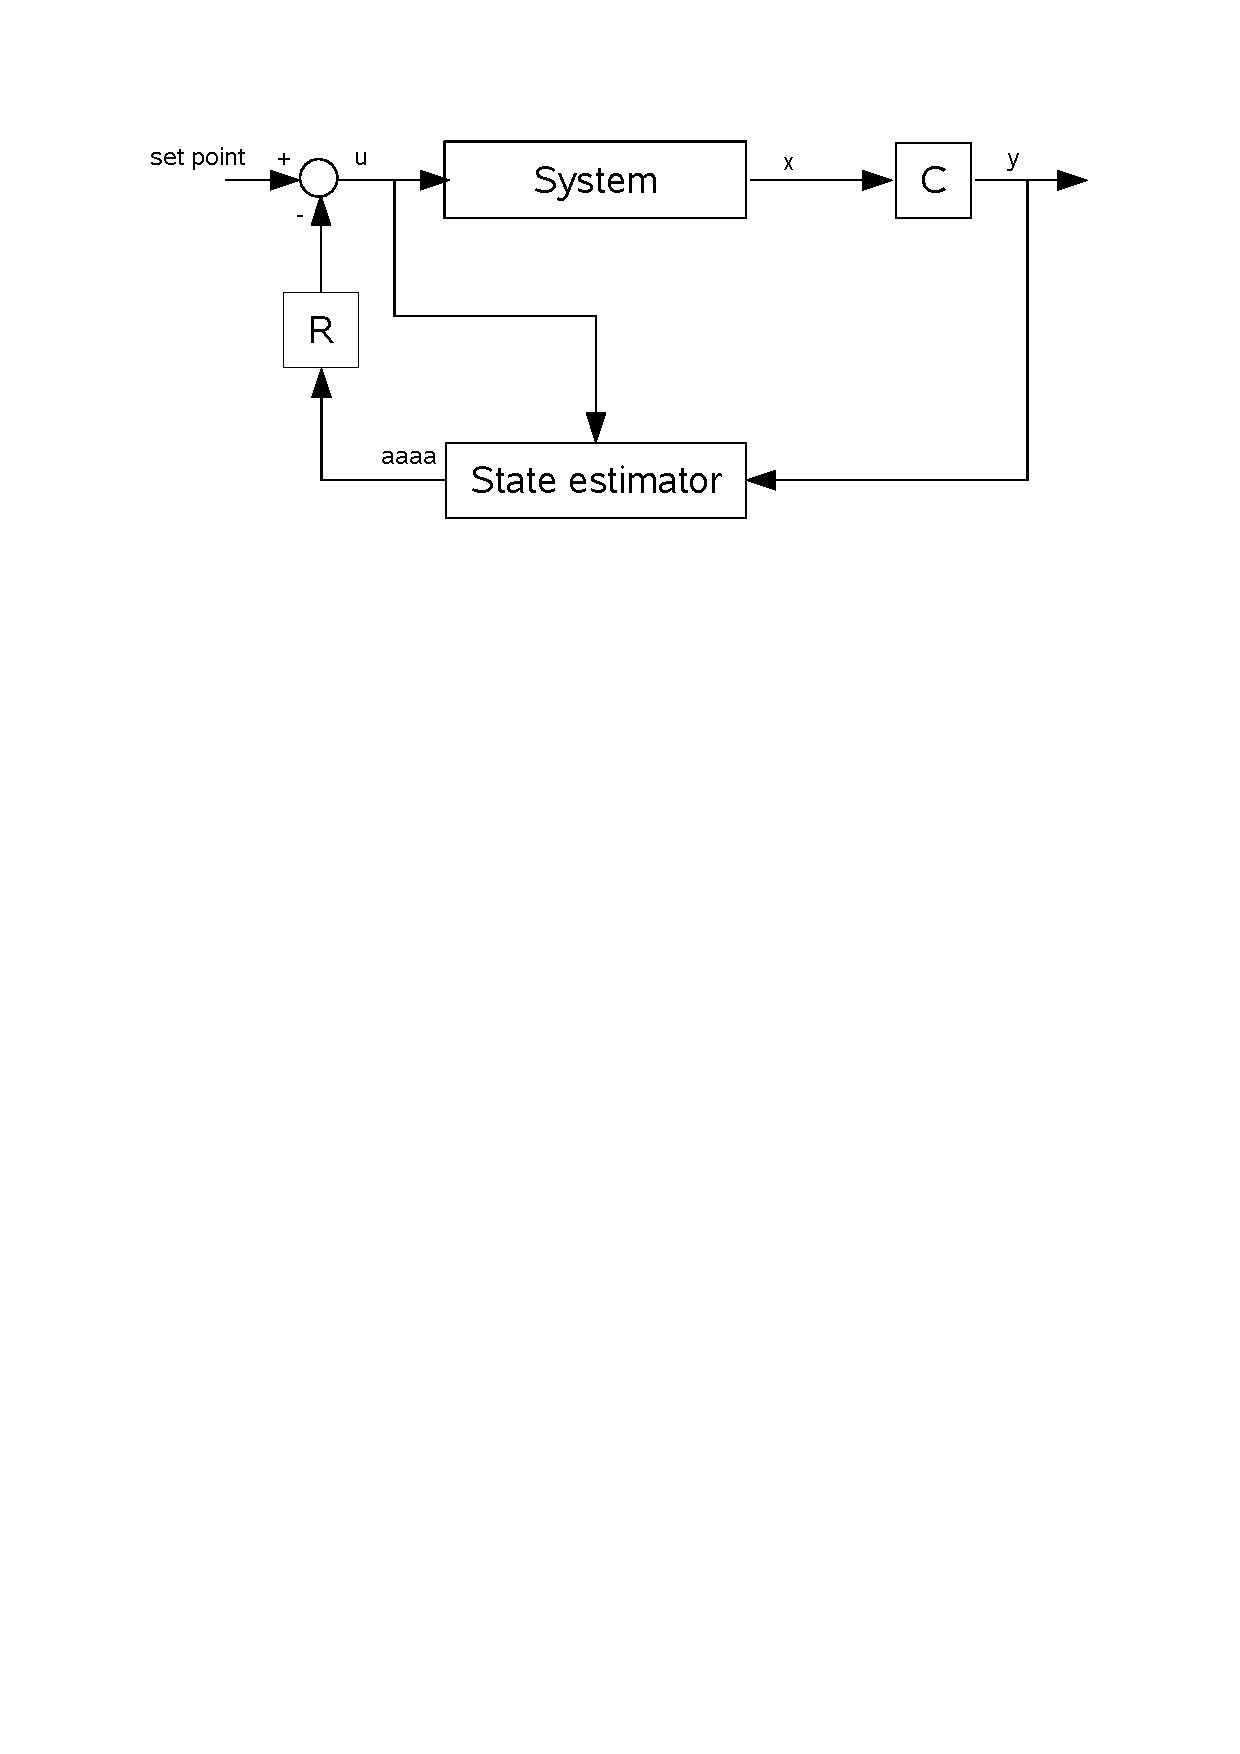
\includegraphics[trim = 10mm 200mm 20mm 20mm, clip,scale=0.80]{Bilder/system_observer.pdf}
\tikzstyle{block} = [draw, fill=blue!20, rectangle, 
    minimum height=3em, minimum width=6em]
\tikzstyle{sum} = [draw, fill=blue!20, circle, node distance=1cm]
\tikzstyle{input} = [coordinate]
\tikzstyle{output} = [coordinate]
\tikzstyle{pinstyle} = [pin edge={to-,thin,black}]
\def\blockdist{2.3}
% The block diagram code is probably more verbose than necessary
\begin{tikzpicture}[auto, node distance=4cm,>=latex']
    % We start by placing the blocks
    \node [input, name=input] {};
    \node [sum, right of=input] (sum) {};
    \node [block, right of=sum] (controller) {Controller};
    \node [block, right of=controller, pin={[pinstyle]above:Disturbances},
            node distance=5cm] (system) {System};
    % We draw an edge between the controller and system block to 
    % calculate the coordinate u. We need it to place the measurement block. 
    \draw [->] (controller) -- node[name=u] {$u$} (system);
    \node [output, right of=system] (output) {};
    \node [block, below of= controller] (measurements) {Estimator};

    % Once the nodes are placed, connecting them is easy. 
    \draw [draw,->] (input) -- node {$r$} (sum);
    \draw [->] (sum) -- node {$e$} (controller);
    \draw [->] (system) -- node [name=y] {$y$}(output);
    \draw [->] (y) |- (measurements.base east);
    \draw [->] (u) |- (measurements.10);
    \draw [->] (measurements) -| node[pos=0.99] {$-$} 
        node [near end] {$\hat{x}$} (sum);
\end{tikzpicture}
    \caption{State feedback controller with state estimator}
      \label{fig:observer}
\end{figure}

The state space equations of a nonlinear system is
\begin{equation}
\begin{split}
\label{eqn:nl_sys}
\dot{x}(t) &= f(x(t),u(t)) , x(t=0) = x_0 \\
y(t) &= g(x(t),u(t)),
\end{split}
\end{equation}

where $t$ is a scalar representing time, $x(t)$ represents the state vector, $u(t)$ represents the input vector and $y(t)$ represents the output vector of the system. The state $x(t)$,input $u(t)$ and output $y(t)$ depends on time $t$. The variable $x_0$ represents the vector of initial states $x(t=0)$ of the system. 
The state space equations of the state estimator is 
\begin{equation}
\begin{split}
\label{eqn:est_sys}
\dot{\hat{x}}(t) &= f(\hat{x}(t),u(t)) + K(y(t)-\hat{y}(t)) , \hat{x}(t=0) = \hat{x}_0  \\
\hat{y}(t) &= g(\hat{x}(t),u(t)),
\end{split}
\end{equation}
where $\hat{x}(t)$ \footnote{ The estimated states are represented by hat symbol at the top, inorder to differentiate them from the true states of the system. For example $\hat x_k$ represents the estimated states} is the state vector of estimator and $K$ is the estimator gain matrix.  A state estimator should satisfy the following properties \citep{gre01}:
\begin{itemize}
\item \textbf{Simulation property:} When the estimator and the system to be observed have same initial condition $x_0 = \hat{x}_0$, then it holds that $x(t) = \hat{x}(t) \forall t > 0 $
\item \textbf{Convergence property:} If $x_0 \neq \hat{x}_0$, then $x(t) - \hat{x}(t)$ tends to zero as $ t \rightarrow \infty $.
\end{itemize}

There are different methods for computing the estimator gain matrix $K$ in Equation \ref{eqn:est_sys}. The Luenberger observer has a deterministic way of computing the gain for linear systems. The sliding mode observer and the Kalman filter determines the gain matrix by minimizing the error between the estimates $\hat{x}$ and actual states $x$ \citep{kha02}.
    \section{Kalman Filter}
Kalman filter is a statistical state estimation algorithm which estimates the internal state of the system from the noisy measurements. It was designed by Rudolph E. Kalman in 1960 for discrete time linear systems. It is basically a predictor-corrector type estimator that is optimal in the sense that it minimizes the estimated error covariance. Since the measurements occur and the states are estimated at discrete points of time, it is easily implementable in digital computers. Kalman filters are extensively used in the area of autonomous and guided navigation.

\subsection{Kalman gain}
Given a discrete time linear system affected by random noise
\begin{equation}
\begin{split}
x_{k} &= Ax_{k-1} + Bu_k + w_{k-1}\\
y_k &= Hx_k + v_k
\end{split}
\end{equation}
where the random variables $w_k$,$v_k$ represent the process and measurement noise. Both the random variables are assumed to be zero mean Gaussian white noises. Let $Q,R$ be the covariance of process and measurement noise. Let us assume, 
\begin{equation}\label{eqn:kf_err}
e_k^- = x_k - \hat{x_k}^- 
\end{equation} be the error between the actual and predicted value of the state. The error covariance is given by 
\begin{equation}\label{eqn:kf_P}
P_k^- = E[e_k^- {e_k^-}^T]
\end{equation} Kalman filter corrects it estimate based on the predicted state and measured output data by 
\begin{equation} \label{eqn:kf_correct}
\hat{x_k} = \hat{x_k}^- + K(y_k - H\hat{x_k}^-)
\end{equation}
Kalman gain is computed by substituting Equation \ref{eqn:kf_correct} in Equation \ref{eqn:kf_err} to compute the $e_k^-$. Computed $e_k^-$ is substituted in Equation \ref{eqn:kf_P} and the expected values are computed to find the error covariance $P_k^-$. Finally \emph{K} is computed by taking the derivative of trace of $P_k^-$ and equating it to zero $$ \dfdx{trace(P_k^-)}{K} = 0 $$ solving the above equation for \emph{K}. One form of \emph{K} that minimizes Equation \ref{eqn:kf_correct}
\begin{equation} \label{eqn:kf_gain}
 K_k = P_k^- H^T(H P_k^- H^T + R)^{-1}
\end{equation}
From the Equation \ref{eqn:kf_gain} as measurement covariance \emph{R} approaches zero, Kalman gain \emph{K} lays more trust on actual measurement $y_k$. On the other hand if $P_k^-$ approaches zero, predicted measurement $H\hat{x_k}^-$ is trusted more.

\subsection{Extended Kalman filter}
Most of the real world estimation scenarios are non linear in nature. Kalman filter algorithm cannot be applied to the non linear systems. \emph{NASA Ames} devised a method to apply Kalman filter for non linear systems which is called the Extended Kalman filter(EKF). In EKF the non linear system is linearised by multivariate Taylor series expansion of the non linear function. 

Given a discrete time non linear system,
\begin{equation}
\begin{split}
x_{k} &= f(x_{k-1},u_k,w_{k-1})\\
y_k &= h(x_k,u_k,v_k)
\end{split}
\end{equation}
\emph{x,y} denotes the vector of system's state and output. \emph{w,v} represents the process and measurement covariance noise. \emph{f} is the non linear function that relates the previous state to the current state and \emph{h} is the non linear function that relates the output and state. 

In practice the individual values of noise $w_k$ and $v_k$ at each time step \emph{k} is not known. So one can compute the approximated state and measurement vector without them as 
\begin{equation}
\begin{split}
\hat{x}_k^- &= f(\hat{x}_{k-1},u_{k},0)\\
\hat{y}_k^- &= h(\hat{x}_k^-,u_{k},0)
\end{split}
\end{equation}
$\hat{x}_k^-$ and $\hat{y}_k^-$ are the \emph{priori} estimates of state and measurements at time step \emph{k} computed from \emph{posteriori} estimate of state $\hat{x}_{k-1}$ from previous time step \emph{k-1}.

$A_k$ and $H_k$ be the Jacobian matrices that results taking partial derivative of \emph{f} and \emph{h} with respect to \emph{x}  at time instant \emph{k}. $W_k$ and $V_k$ be the Jacobian matrices that results taking partial derivative of \emph{f} with respect to \emph{w} and \emph{h} with respect to \emph{v} at time step \emph{k}.
\begin{equation}
\begin{split}
A_k(i,j) &= \dfdx{f_i}{x_j}(\hat{x}_{k-1},u_k,0)\\
C_k(i,j) &= \dfdx{h_i}{x_j}(\hat{x}_k^-,u_k,0)\\
W_k(i,j) &= \dfdx{f_i}{w_j}(\hat{x}_{k-1},u_k,0)\\
V_k(i,j) &= \dfdx{h_i}{v_j}(\hat{x}_k^-,u_k,0)\\
\end{split}
\end{equation}
At each time step these Jacobian matrices are evaluated with current predicted states $\hat{x}_k^-$.
\subsubsection{Algorithm}
\textbf{Predict}
\begin{equation}
\begin{split}
%\text{Project the state}\\
\hat{x}_k^- &= f(\hat{x}_{k-1},u_k,0)\\
%\text{Procject the covarience}\\
P_k^- &= A_kP_{k-1}A_k^T + W_kQ_{k-1}W_k^T\\
\end{split}
\end{equation}
\textbf{Correct}\\
\begin{equation}
\begin{split}
K_k &= P_k^-H^T(H_kP_k^-H_k^T + V_kR_kV_k^T)^{-1}\\
\hat{x}_k &= \hat{x}_k^- + K_k(y_k-h(x_k^-,u_k,0))\\
P_k &= (I- K_kH_k)P_k^-
\end{split}
\end{equation}
% The result of th It has to be extended is  non-linear systems by extending the actual algorithm. This type of kalman filter algorithms %are called Extended kalman filters. There are also a new class of kalman filter algorithm which works on Bayasian principle, they are %called unscented Kalman filters.
\subsection{Unscented Kalman filter}
    %\chapter{Conclusion}
\label{ch:conclusion}

%Filter Comparison:
 The state estimation problem is solved with the EKF and the UKF. The EKF involves more modeling than the UKF. For example modeling of the Jacobian matrices $A$ and $C$ for multibody model of \emph{Toro} in Chapter \ref{ch:multi_mdl}. The UKF is easier to tune for models with less number of states (IDP) than for the models with many states (\emph{toro}). The computation time of the UKF is higher than the EKF for all the models. 
 \begin{table}[H]
	\centering
	\setlength{\extrarowheight}{0.5cm}
%\setlength{\extrarowwidth}{0.1cm}
\begin{tabular}{|x{1cm}|x{2cm}|x{2.1cm}|}\hline
Model&RMSE&Computation time\\ \hline
IDP&\diag{0.25em}{2cm}{ 
\includegraphics[scale=0.025]{Bilder/thumbs-up.png} }{
\includegraphics[scale=0.025]{Bilder/thumbs-up.png}}&\diag{0.25em}{2cm}{
\includegraphics[scale=0.025]{Bilder/thumbs-up.png}}{
\includegraphics{Bilder/thumbs-down.png}} \\ \hline
Toro&\diag{0.25em}{2cm}{
\includegraphics[scale=0.025]{Bilder/thumbs-up.png}}{
\includegraphics{Bilder/thumbs-down.png}}&\diag{0.25em}{2cm}{
\includegraphics[scale=0.025]{Bilder/thumbs-up.png}}{
\includegraphics{Bilder/thumbs-down.png}}\\ \hline
IMU&\diag{0.25em}{2cm}{
\includegraphics[scale=0.025]{Bilder/thumbs-up.png}}{-}&\diag{0.25em}{2cm}{
\includegraphics[scale=0.025]{Bilder/thumbs-up.png}}{-}\\ \hline
\end{tabular}

	\caption{Comparison of qualitative performance of EKF and UKF on the models}
	\label{tab:comp_ekf_ukf}
\end{table}

The smiley \footnote{Smiley image source:\url{http://www.clker.com/}.} on the left side of each cell in Table \ref{tab:comp_ekf_ukf} refers to the performance of EKF, whereas the one on the right side of refers to UKF. Since the UKF was not developed for the IMU model the RMSE is left blank. 

%Models Comparison:
The state estimation problem is approached with multibody system model of \emph{Toro} and the model of IMU. The EKF has same performance with both models which can be inferred from the RMSE values of the estimates in Tables \ref{tab:toro_rmse} and \ref{tab:simp_rmse}. The computation time of EKF for the \emph{Toro} model is higher than the IMU model. This makes the \emph{Toro} model inapplicable for real time applications. Whereas the IMU model having low computation time is implemented on the real robot.

\begin{table}
	\centering
	%\setlength{\extrarowheight}{0.5cm}
	%\begin{tabular}{|x{1cm}|x{2cm}|x{2cm}|}\hline
	\begin{tabular}{|c|c|c|}\hline
	&Toro&IMU \\ \hline	
	RMSE &
\includegraphics[scale=0.025]{Bilder/thumbs-up.png}&
\includegraphics[scale=0.025]{Bilder/thumbs-up.png} \\ \hline
	Computation time &
\includegraphics{Bilder/thumbs-down.png} &
\includegraphics[scale=0.025]{Bilder/thumbs-up.png} \\ \hline
	\end{tabular}
	\caption{Comparison of qualitative performance of the models used in EKF }
\end{table}

The multibody model of \emph{Toro} is more descriptive and complicated than the IMU model. It is possible to estimate additional motion parameters like joint velocities $\dot q$ with this model, but it is computationally costly. This model is prone to modeling errors. The IMU model is simpler than multibody model and computationally cheap. The formulation of the model is easier than \emph{Toro} model. This model have the same performance as the \emph{Toro} model.

\subsection{Future works}
The filters designed in this thesis are aimed to be used in the controllers for balancing applications in \emph{Toro}. But this can be extended for walking applications in the future. The camera present at the head of \emph{Toro} provides measurements at lower frequency (100Hz) than the other sensors (1kHz). The could be incorporated as additional measurement \citep{vis12}.

    %%%%%%%%%%
    % Anhang %
    %%%%%%%%%%

    \appendix
	%\printindex
    %Abbildungsverzeichnis
    \listoffigures
    \addcontentsline{toc}{chapter}{List of figures}
    %\addcontentsline{lof}{figure}{List of figures}
    \cleardoublepage
    %list of tables
    %\listoftables
    %\addcontentsline{lot}{tables}{List of tables}
    % Literaturverzeichnis
    \addcontentsline{toc}{chapter}{\bibname}
    %\bibliographystyle{gerplain}
    %\bibliographystyle{unsrt}
    \bibliographystyle{alphadin}
    \bibliography{literatur}
		
    % Erklaerung
    \newpage
    \thispagestyle{myheadings}
    \markboth{}{ERKL\"{A}RUNG}
    \addcontentsline{toc}{chapter}{Erkl\"{a}rung}
    % erklaerung.tex
% Stand 31.08.2011

\cleardoublepage
\begin{center}
\textbf{Eidesstattliche Versicherung}
\end{center}
\normalsize
% Eventuell anzupassen
%\vspace{2cm}
\begin{table}[H]
	\begin{tabular}{p{10cm} p{5cm}}
	\underline{Rajendran, Rajesh} & 	\underline{146073\hspace{1cm}} \\
	Name, Vorname  &Matrikel-Nr.
	\end{tabular}
\end{table}
Ich versichere hiermit an Eides statt, dass ich die vorliegende \underline{Masterarbeit} mit dem Titel \\
\begin{center}
\textbf{\underline{"Estimation of underactuated degrees of freedom in humanoid robots"}}
\end{center}
%\hrulefill \\ \hrule \hrule
%\hrulefill \\ \hrule  \hrule
\vspace{0.5cm}
selbstst�ndig und ohne unzul�ssige fremde Hilfe erbracht habe. Ich habe keine anderen als die angegebenen Quellen und Hilfsmittel benutzt sowie w�rtliche und sinngem��e Zitate kenntlich gemacht. Die Arbeit hat in gleicher oder �hnlicher Form noch keiner Pr�fungsbeh�rde vorgelegen.\\
%\vspace{2cm}
\normalsize
\begin{table}[H]
	\begin{tabular}{p{10cm} p{5cm}}
	\underline{Dortmund,den \today} & 	\underline{\hspace{3cm}} \\
	Ort, Datum  &Unterschrift.
	\end{tabular}
\end{table}

\textbf{Belehrung:} 

Wer vors�tzlich gegen eine die T�uschung �ber Pr�fungsleistungen betreffende Regelung einer Hochschulpr�fungsordnung verst��t, handelt ordnungswidrig. Die Ordnungswidrigkeit kann mit einer Geldbu�e von bis zu 50.000,00 Euro geahndet werden. Zust�ndige Verwaltungsbeh�rde f�r die Verfolgung und Ahndung von Ordnungswidrigkeiten ist der Kanzler der Technischen Universit�t Dortmund. Im Falle eines mehrfachen oder sonstigen schwerwiegenden T�uschungsversuches kann der Pr�fling zudem exmatrikuliert werden. (� 63 Abs. 5 Hochschulgesetz - HG - )\\

Die Abgabe einer falschen Versicherung an Eides statt wird mit Freiheitsstrafe bis zu 3 Jahren oder mit Geldstrafe bestraft.\\

Die Technische Universit�t Dortmund wird gfls. elektronische Vergleichswerkzeuge (wie z.B. die Software "turnitin") zur �berpr�fung von Ordnungswidrigkeiten in Pr�fungsverfahren nutzen.\\

Die oben stehende Belehrung habe ich zur Kenntnis genommen:\\
\begin{table}[H]
	\begin{tabular}{p{10cm} p{5cm}}
	\underline{Dortmund,den \today} & 	\underline{\hspace{3cm}} \\
	Ort, Datum  &Unterschrift.
	\end{tabular}
\end{table}
\begin{comment}
%Hiermit best�tige ich, die vorliegende Diplomarbeit selbst�ndig und nur unter Zuhilfenahme
%der angegebenen Literatur verfasst zu haben.
\setlength{\parskip}{50pt}
\par
% In manchen Studieng�ngen optional. Gegebenenfalls l�schen.
Ich bin damit einverstanden, dass Exemplare dieser Arbeit in den Bibliotheken der
Universit�t Dortmund ausgestellt werden. 
\setlength{\parskip}{50pt}
\par
Dortmund, den \today 
\setlength{\parskip}{50pt}
\par
Name
\end{comment}
\clearpage
% EOF

%%%%%%%
% END %
%%%%%%%
\end{document}



